\documentclass[grad,pdftex,numbers]{coppetex/coppe}
\usepackage{amsmath,amssymb}
\usepackage{hyperref}
\usepackage[utf8]{inputenc}

\usepackage{listings}
\usepackage{color}

\lstset{frame=tb,
  language=Java,
  aboveskip=3mm,
  belowskip=3mm,
  showstringspaces=false,
  columns=flexible,
  basicstyle={\small\ttfamily},
  numbers=none,
  numberstyle=\tiny\color{gray},
  keywordstyle=\color{blue},
  commentstyle=\color{dkgreen},
  stringstyle=\color{mauve},
  breaklines=true,
  breakatwhitespace=true,
  tabsize=3
}
\definecolor{dkgreen}{rgb}{0,0.6,0}
\definecolor{gray}{rgb}{0.5,0.5,0.5}
\definecolor{mauve}{rgb}{0.58,0,0.82}

\makelosymbols
\makeloabbreviations

\begin{document}
  \title{Desenvolvimento de Aplicativos Android e iOS para o Restaurante Universit\'ario da UFRJ}
  \foreigntitle{Thesis Title}
  \author{Felipe}{Podolan Oliveira}
  \advisor{Prof.}{Nome do Primeiro Orientador}{Sobrenome}{D.Sc.}
  \advisor{Prof.}{Nome do Segundo Orientador}{Sobrenome}{Ph.D.}
  \advisor{Prof.}{Nome do Terceiro Orientador}{Sobrenome}{D.Sc.}

  \examiner{Prof.}{Nome do Primeiro Examinador Sobrenome}{D.Sc.}
  \examiner{Prof.}{Nome do Segundo Examinador Sobrenome}{Ph.D.}
  
  
  \department{PESC}
  \date{11}{2018}

  \keyword{Primeira palavra-chave}
  \keyword{Segunda palavra-chave}
  \keyword{Terceira palavra-chave}

  \maketitle

  \dedication{Este trabalho é dedicado aos meus pais}

\chapter*{Agradecimentos}

Quando eu tinha 16 anos, eu resolvi sair de casa para estudar. 
Foi uma decisão difícil que daria início a uma jornada igualmente difícil. Minha vida mudou 
completamente sem meus pais e sem minha irmã ao meu lado em uma cidade completamente diferente
da cidade em que eu nasci no interior do Paraná. Desde então, eu passei alguns anos fazendo 
cursinho preparatório em São José dos Campos - SP para o ITA (Instituto Tecnológico da Aeronáutica.
Até que em 2012, eu resolvi desistir e prestei vestibular para a UFRJ.

Em todas minhas decisões, minha mãe e meu pai sempre me apoiaram seja com conselhos, 
com apoio moral ou financeiro. Durante minha vida acadêmica na UFRJ e fora dela, eu passei
por diversas dificuldades e meus pais sempre estiveram do meu lado.

Agradeço a eles pelo suporte, pelo carinho e pela educação que eles me deram. 
Meus pais sempre serão meus exemplos de vida, de como ser como pessoa.

Eu também agradeço à minha irmã, ao meu cunhado e ao meu sobrinho pelo amor e carinho 
que sempre me deram e também aos meus amigos que sempre se mostraram dispostos a me ajudar.

Agradeço à UFRJ, como instituição, que foi quase como um segundo lar por alguns 
anos e me proporcionou diversas oportunidades únicas, como o intercâmbio através 
do programa Ciências sem Fronteiras, em 2015 e 2016.

Por fim, agradeço aos meus professores que contribuíram para a minha formação e por passarem
o conhecimento necessário para eu me tornar um engenheiro.

  \frontmatter
  \tableofcontents
  \listoffigures
  \listoftables
  \printlosymbols
  \printloabbreviations

  \mainmatter
  \chapter{Introdução}

O Restaurante Universitário da UFRJ tem como objetivo oferecer alimentação de qualidade, equilibrada, e 
acessível de forma a favorecer a permanência dos estudantes no espaço universitário, permitindo-lhes 
dedicação integral aos estudos, sendo importante meio de combate à evasão escolar.

Entretanto, apesar de ser benéfico à comunidade universitária, o RU enfrenta alguns problemas, sendo o 
principal as filas de espera. Pensando nisso, a Decania do Centro de Tecnologia resolveu criar um sistema
 de agendamento online cujo objetivo é alocar os horários de entrada no RU.

Esse projeto funciona desde 2016 na unidade do RU do CT. Os agendamentos são feitos através do website
www.ru.ct.ufrj.br. Entretanto, para melhorar ainda mais a experiência dos usuários, a Decania do CT 
resolveu desenvolver aplicativos para smartphone tendo em vista a crescente popularização desta 
plataforma, notoriamente para Android e para iOS.

Desde então, eu ingressei no projeto com o intuito de desenvolver esses aplicativos nativos. Esta 
monografia mostrará um comparativo entre essas duas ferramentas e utilizará como ilustração
os aplicativos desenvolvidos para o Restaurante Universitário da UFRJ.
  \chapter{Interface Gráfica (UI)}

\section{Android}
\subsection{Activities}
A plataforma Android oferece algumas opções de criação de interfaces telas. A principal maneira de 
fazê-lo é utilizando uma classe nativa chamada Activity. A classe Activity é responsável por carregar uma 
user interface (UI) é definida através de um arquivo XML de layout usualmente guardado no diretório 
/res/layout do projeto.

No exemplo a seguir, modificado do projeto RestauranteUniversitário, a classe MainActivity herda da classe
AppCompactActivity (um dos tipos de Activity fornecidas pelo Android), e carrega a user interface 
activity\_main.


\lstset{language=Java}

\begin{lstlisting}
// MainActivity.java

package br.ufrj.ct.restauranteuniversitario;

import android.os.Bundle;
import android.support.v7.app.AppCompatActivity;

public class MainActivity extends AppCompatActivity {
    
    @Override
    protected void onCreate(Bundle savedInstanceState) {
        super.onCreate(savedInstanceState);

        //set the layout from the res/layout folder
        setContentView(R.layout.activity_main);
        
     }
}

\end{lstlisting}

Note que o método onCreate é chamado quando a Activity é criada. Ainda mais, existe 
todo um ciclo de vida que define o comportamento de uma Activity dada a interação dela com o 
usuário, conforme mostrado na figura a seguir.

\begin{figure}[htb]
    \centering
    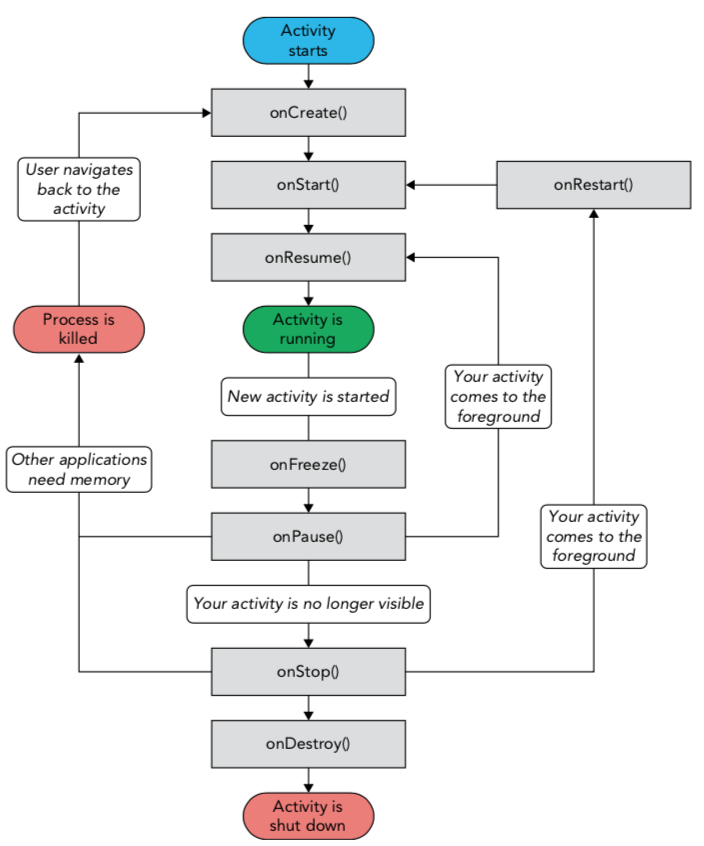
\includegraphics[width=\textwidth]{images/android_activity_lifecycle}
    \caption[Exemplo de detecção das trilhas de transformações]
    {Ciclo de vida de uma Activity do Android.}%
    \label{fig:android_activity_lifecycle}
\end{figure}




  \backmatter
  \bibliographystyle{coppe-unsrt}
  \bibliography{example}

  \appendix
  \chapter{Algumas Demonstra{\c c}\~oes}
\end{document}
